\chapter{Results}
% This should be 3000 words split with the methods

\section{Response Times \& Task Construction Verification}
\begin{table}[hbt!]
    \begin{center}
        \caption{Tabulated Values of Number of Decisions Presented to the Subjects}
        \begin{tabular}{|c|c|c|c|c|}
        \hline
        Subject &   Cyclist Decisions   & Car Decisions & Missed Decisions & Total Decisions \\ \hline
        a       &   57  & 53    & 7     & 117   \\ \hline
        b       &   55  & 47    & 5     & 107   \\ \hline
        c       &   62  & 60    & 7     & 129   \\ \hline
        d       &   40  & 46    & 7     & 93    \\ \hline
        e       &   64  & 65    & 2     & 131   \\ \hline
        f       &   50  & 54    & 10    & 114   \\ \hline
        g       &       &       &       &       \\ \hline
        \end{tabular}
    \end{center}
\end{table}


% Summary Reaction Time Results
\begin{table}[hbt!]
    \begin{center}
        \caption{Tabulated Values of Reaction Time for Each Subject}
        \begin{tabular}{|c|c|cc|cc|}
        \hline
        \multirow{2}{*}{Subject} & \multirow{2}{*}{Overall Mean} & \multicolumn{2}{c|}{Cyclist Mean} & \multicolumn{2}{c|}{Car Mean}  \\ \cline{3-6} 
                                &           & Overtaking    & Slowing Down  & Overtaking & Slowing Down \\ \hline
        a                       &   2.92    & 4.70          & 2.76          & 3.40      &   1.44        \\ \hline
        b                       &   1.90    & 4.52          & 2.30          & 3.13      &   0.85        \\ \hline
        c                       &   2.87    & 5.29          & 2.78          & 0.51      &   1.87        \\ \hline
        d                       &   2.16    & 3.31          & 1.56          & 0.77      &   1.53        \\ \hline
        e                       &   2.14    & 3.42          & 2.12          & 2.28      &   0.90        \\ \hline
        f                       &   2.17    & 3.97          & 2.72          & 0.52      &   1.13        \\ \hline
        g                       &           &               &               &           &               \\ \hline
        \end{tabular}
    \end{center}
\end{table}

\begin{figure}[hbt!]
    \centering
    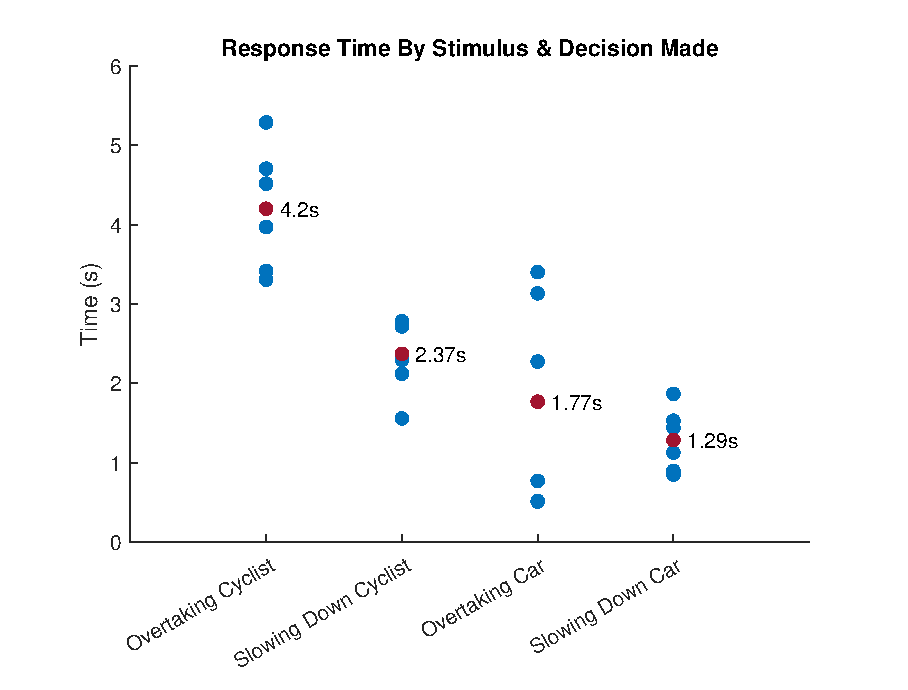
\includegraphics[width=0.75\linewidth]{figures/ReactionTimeMean.eps}
    \caption{}
    \label{fig:RT_Total}
\end{figure}

% Response Time Plots
\begin{figure}[hbt!]
    \centering
    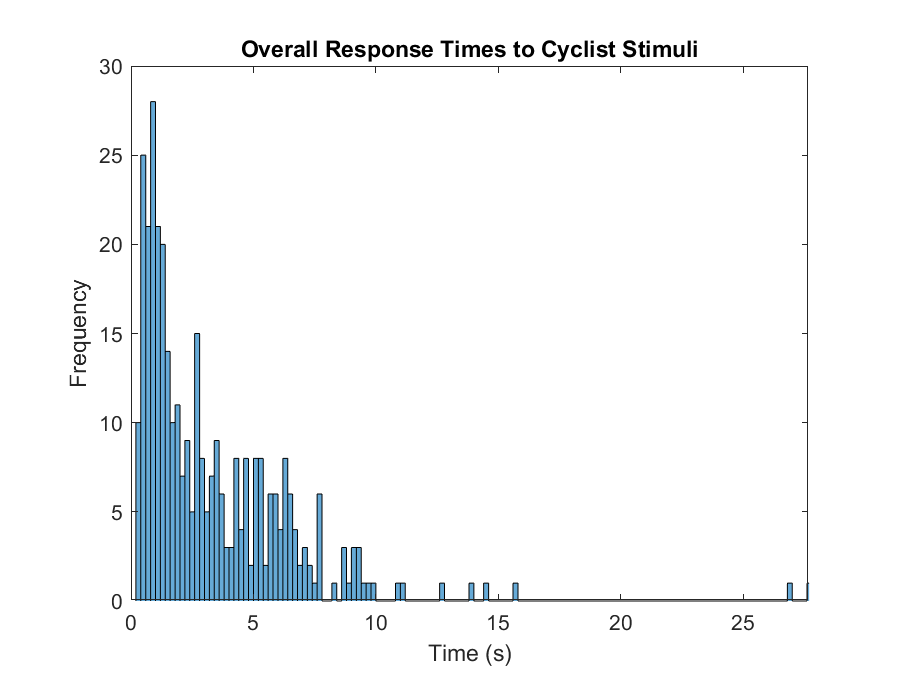
\includegraphics[width=0.45\linewidth]{figures/BikeReactionTimes.eps}
    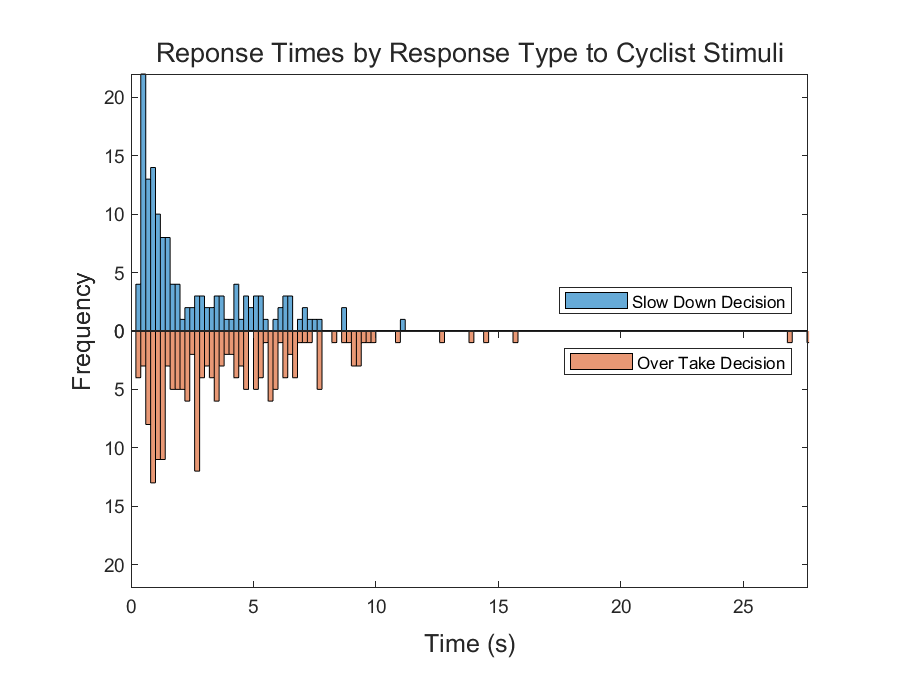
\includegraphics[width=0.45\linewidth]{figures/BikeReactionTimes2.eps}
    \caption{Non-Subject Specific Distribution of Response times to the 'Cyclist' Stimulus. a) Not Segregated by Response Type b) Segregated by Response Type}
    \label{fig:RT_B}
\end{figure}

\begin{figure}[hbt!]
    \centering
    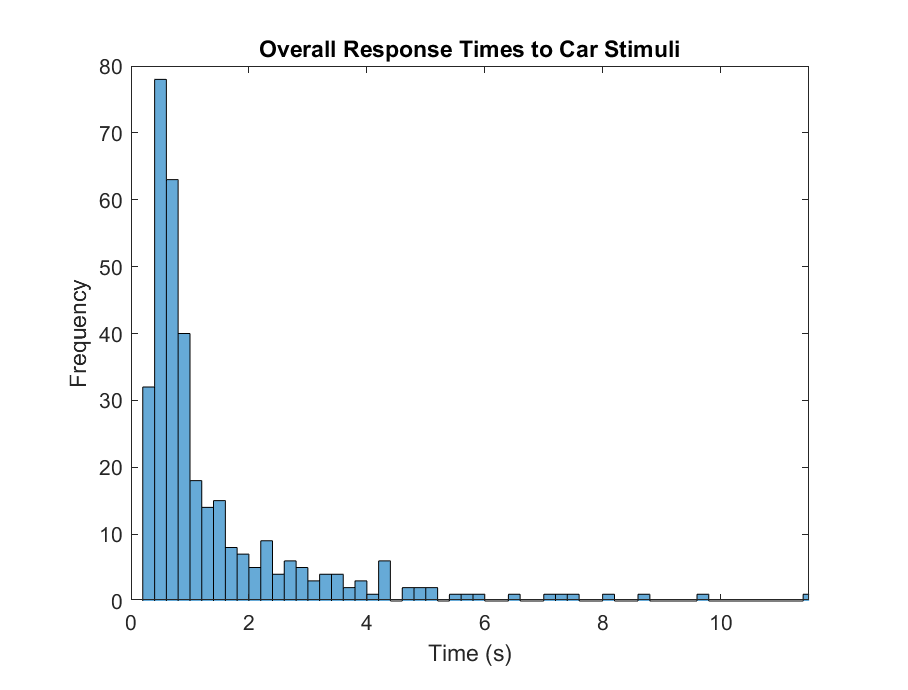
\includegraphics[width=0.45\linewidth]{figures/CarReactionTimes.eps}
    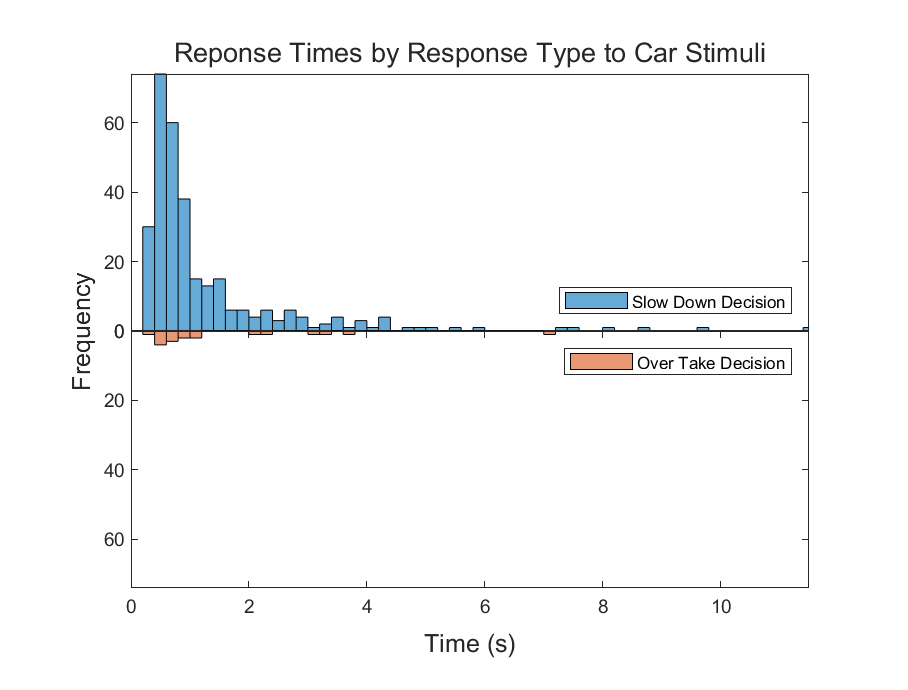
\includegraphics[width=0.45\linewidth]{figures/CarReactionTimes2.eps}
    \caption{Non-Subject Specific Distribution of Response times to the 'Car' Stimulus. a) Not Segregated by Response Type b) Segregated by Response Type}
    \label{fig:RT_C}
\end{figure}

As can be clearly seen in figure \ref{fig:RT_C} the number of 'incorrect' overtake responses to the 'Car' stimuli is negligible. Using this 